
\subsection{Build an interesting grammar by hand}

\experiment{1.grammars/handbuilt/handbuilt.py}

Here we are drawing a grammar. We have built this grammar by hand, by
taking the following curve, and specifying a decomposition of it:

\begin{figure}
\includegraphics[width=\linewidth]{experiments/1.grammars/hand_built/output.d/hand_built_curve.png}
\caption{The initial curve}
\end{figure}

Here is the decomposition:
\begin{figure}
\includegraphics[width=\linewidth]{experiments/1.grammars/hand_built/output.d/hand_built_sdf.png}
\end{figure}

Here is the grammar:

Here are some samples from the grammar:

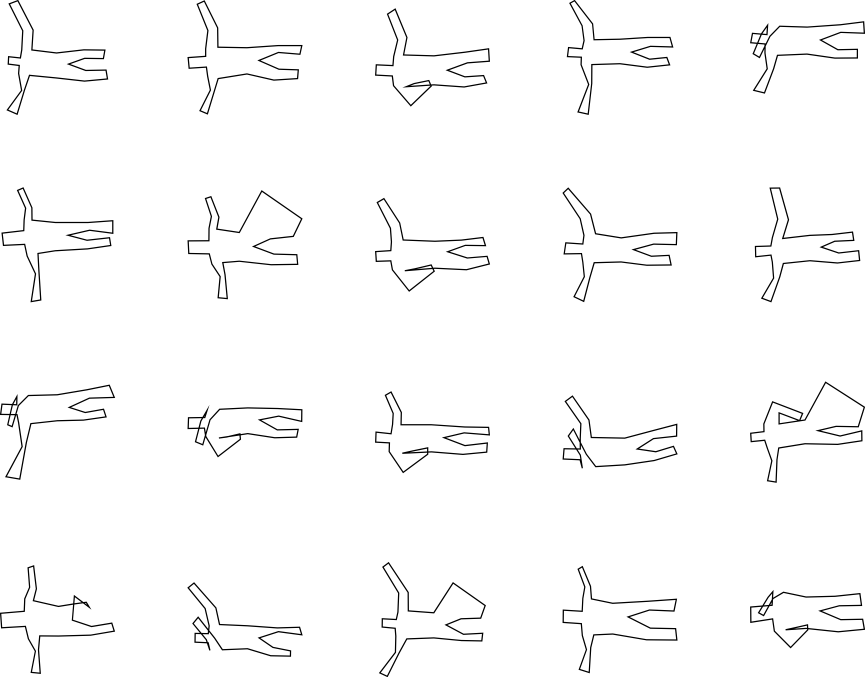
\includegraphics[width=6in]{output/3.learning/incremental/gram.19.d/samples.png}


